\section{Metodologi Penelitian}
\subsection{Pencitraan Airfoil}
\begin{frame}
  Pencitraan airfoil dilakukan melalui pengolahan citra dengan \textit{OpenCV} untuk mengekstrak/mendapatkan suatu pola tertentu \cite{druzhkov2011new}.\\~\\
  \pause

  Pencitraan ini diperlukan dalam membangun model AI dengan arsitektur \textit{CNN} \cite{albawi2017understanding}.\\~\\
\end{frame}

\subsection{Peningkatan Citra Airfoil}
\begin{frame}
    \begin{columns}[t]% instead of multicols
    \begin{column}{.5\linewidth}
      \begin{figure}[h]
        \centering
        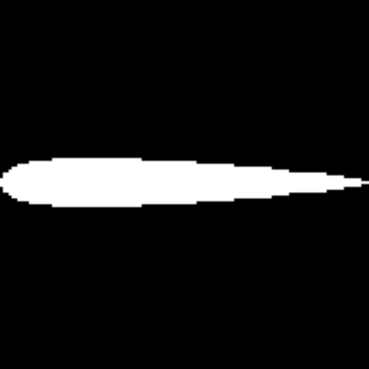
\includegraphics[width=0.5\linewidth]{statics/biner}
        \caption{Citra Biner}
        \label{fig:biner}
      \end{figure}
    \end{column}
    \begin{column}{.5\linewidth}
      \begin{figure}[h]
        \centering
        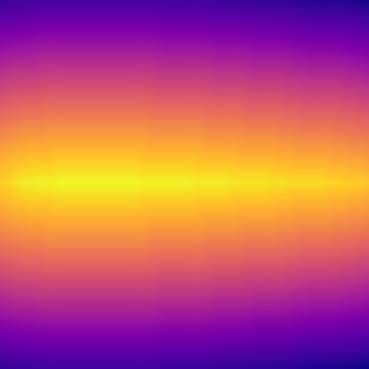
\includegraphics[width=0.5\linewidth]{statics/sdf}
        \caption{Citra SDF}
        \label{fig:biner}
      \end{figure}
    \end{column}
  \end{columns}

  Data geometri dan sudut serang airfoil dapat diubah ke dalam bentuk citra biner. Namun memiliki sedikit variasi piksel. \\~\\

  \pause

  Agar semakin efektif dalam melatih model untuk \textit{CNN}, citra airfoil dibuat dalam bentuk \textit{Signed Distance Fields} (SDF) \cite{guo2016convolutional}.\\~\\
\end{frame}

\subsection{Aerodinamika Airfoil}
\begin{frame}
  Disamping data SDF airfoil, diperlukan data aerodinamika airfoil.\\~\\
  \pause

  Data aerodinamika dapat diperoleh baik melalui pengujian di terowongan angin maupun \textit{CFD}. Penelitian ini menggunakan \textit{CFD} karena lebih murah \cite{eppler2012airfoil}.\\~\\
  \pause

  Banyak \textit{CFD Solver} yang disediakan dalam melakukan analisis aerodinamika airfoil \cite{gunel2016comparison}.
\end{frame}
